%-----------------------------------------------------------------
%	DISTRIBUCIÓ DE LES GALÀXIES A GRAN ESCALA
%	!TEX root = ./../main.tex
%-----------------------------------------------------------------
\section{Distribució de les galàxies a gran escala}
\subsection{Forma i edat de l'Univers}
\subsubsection*{La paradoxa d'Olbers (1829)}
Suposem un Univers infinit amb les estrelles distribuïdes uniformement. Considerem el cel nocturn. El nombre $N$ d'estrelles en una esfera de radi $r$ centrada a la Terra serà
\begin{align}
	N \propto r^{2}
\end{align}
i el flux de radiació rebut a la Terra de cadascuna d'aquestes esferes serà
\begin{align}
	F \propto \frac{1}{r^{2}}
\end{align}
Llavors, $NF = cte$ serà el flux rebut a la Terra a causa de les estrelles en aquesta superfície. En un univers infinit hi hauria un nombre il·limitat d'aquestes superfícies, de manera que el flux total divergiria i el cel nocturn hauria de ser al menys tan lluminós com el diürn.

Aquesta paradoxa ens indica que es compleix alguna de les següents hipòtesis:
\begin{itemize}
	\item L'Univers no és infinit en extensió.
	\item L'Univers no s'expandeix, per la qual cosa la llum de les estrelles pateixen un desplaçament cap al roig proporcionant-nos menys llum que en un Univers estàtic.
	\item Les estrelles no han existit sempre.
\end{itemize}
En definitiva, l'idea d'un Univers infinit i etern (és a dir, sense començament) no és sostenible.

\subsubsection*{L'expansió de l'Univers}
L'any 1923 Edwin Hubble va demostrar que la galàxia M31 (Andròmeda) es troba més enllà de la Galàxia.

Les galàxies es presenten aïllades (\textit{field galaxies}) o formant part d'un grup que pot ser petit (grup, varies dotzenes, com és el cas del nostre Grup Local), mitjanes (cúmuls, centenars), o molt grans (supercúmuls, possiblement una agrupació de cúmuls).

Les estructures de major mida observades fins a la data són aproximadament de $\SI{100}{\mega\parsec}$, clarament més petites que el volum d'espai explorat ($\sim$ varis milers de $\si{\mega\parsec}$).

La distribució de galàxies se sol estudiar cantant el nombre $N(m)$ de galàxies més brillants que la d'una magnitud $m$ donada (figura \ref{fig:N-magnitud}).

Si les galàxies estiguessin distribuïdes uniformement, tindríem que
\begin{align}
	N(<m) \sim 10^{0.6 m}
\end{align}

Efectivament, suposem que totes les galàxies posseeixen la mateixa magnitud absoluta $M$. La distància, en parsecs, ve donada per
\begin{align*}
	d = 10^{(m - M +5 )/5} \si{\parsec}
\end{align*}

\begin{figure}[H]
	\centering
	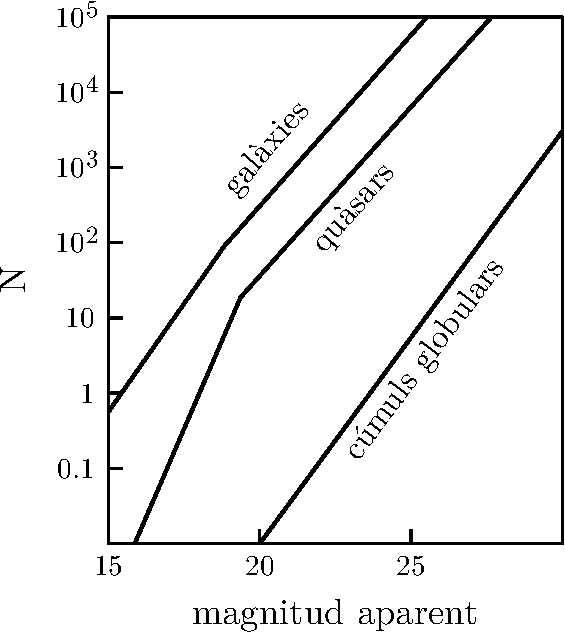
\includegraphics[width=0.4\textwidth]{./images/9-N-magnitud}
	\caption{El canvi de pendent a partir de la magnitud 18 pot entendre's a causa de l'expansió de l'Univers}
	\label{fig:N-magnitud}
\end{figure}

Així, per poder veure una estrella de lluminositat $m$ o major (menor $m$) s'ha de trobar dins d'una esfera de radi $d$ centrada a la Terra.

Com que la distribució de galàxies se suposa uniforme, el seu nombre $N$ serà proporcional a $d^{3}$, és a dir,
\begin{align}
	N \propto d^{3} \propto 10^{0.6 m}
\end{align}
Aquest resultat és independent de la magnitud absoluta $M$, llavors és també vàlid quan les magnituds absolutes difereixen entre si.

L'estudi realitzat per Hubble (1934) basat en aproximadament $\num{44000}$ galàxies indicava una distribució homogènia i isòtropa il·limitada (sense fronteres). Estudis anàlegs sobre radiofonts extragalàctiques mostren que les radiofonts eren més brillants o més nombroses al passat. Això indica que l'Univers no és estàtic sinó que evoluciona.

\subsubsection*{La llei de Hubble (1929)}
Les línies espectrals de les galàxies llunyanes es troben desplaçades cap al roig (figura \ref{fig:galaxies-spectra}) tant més com més distant es troba la galàxia en qüestió:
\begin{align}
	\Delta \lambda \equiv \lambda_{obs} - \lambda_{em} \approx \frac{H_{0}}{c} r \lambda_{em}
\end{align}
on $H_{0}$ és la constant de Hubble ($\approx \SI{70}{\km \per\s \per\mega\parsec}$) i $r$ la distància a la galàxia.
\begin{figure}[H]
	\centering
	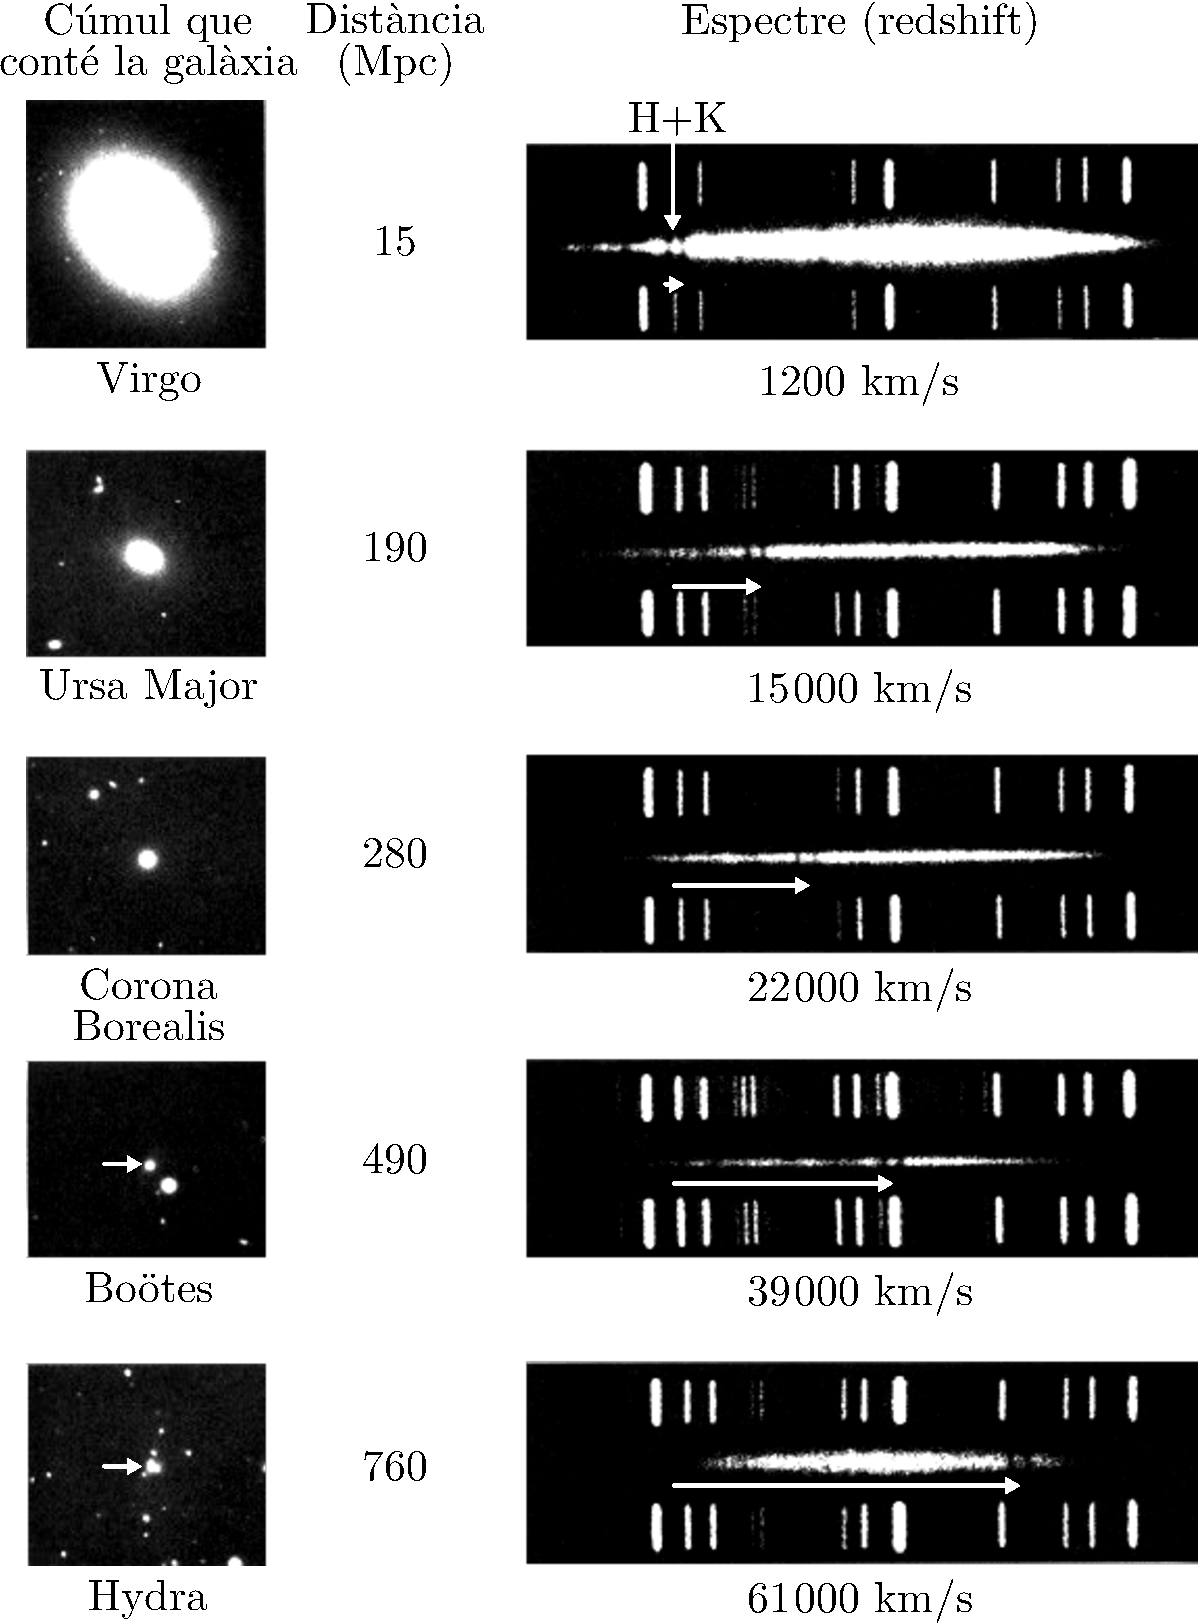
\includegraphics[width=0.7\textwidth]{./images/9-galaxies-spectra}
	\caption{Fotografies i espectres (redshifts) de galàxies localitzades a diferents cúmuls; relació entre el redshitf i la distància
per a galàxies remotes}
	\label{fig:galaxies-spectra}
\end{figure}

En termes del redshift, la llei de Hubble s'escriu
\begin{align}\label{eq:hubble-law}
	z = \frac{H_{0}}{c} r
\end{align}
Si el desplaçament és cap al roig és degut a l'efecte Doppler, llavors $z = v/c$, aleshores
\begin{align}
	v = H_{0} r
\end{align}
Aquest fet se sol interpretat com l'expansió de l'Univers (figura \ref{fig:hubble-diagram}).
\begin{figure}[h]
	\centering
	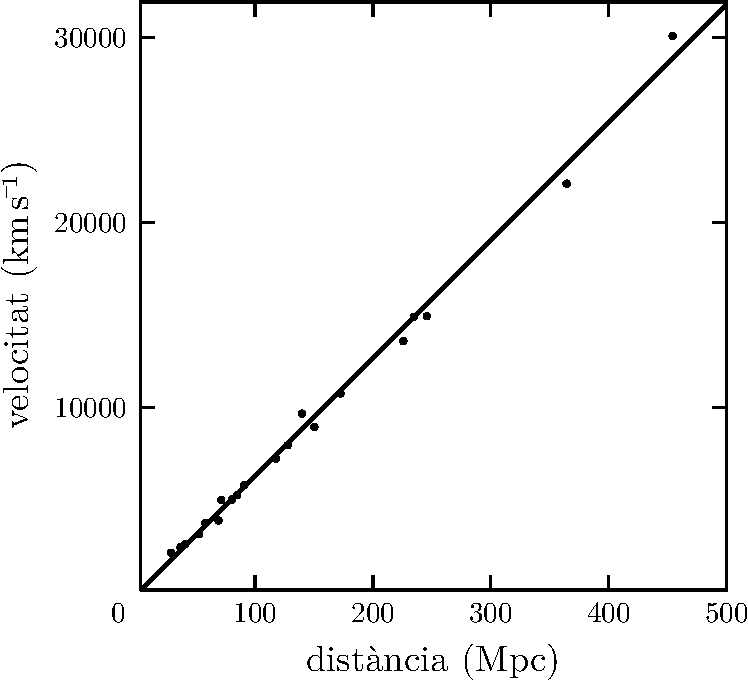
\includegraphics[width=0.55\textwidth]{./images/9-hubble-diagram}
	\caption{Diagrama de Hubble mostrant la correlació entre el redshift (eix $y$) i un indicador de distància basat en cúmuls el·líptics de primera classe (eix $x$)}
	\label{fig:hubble-diagram}
\end{figure}

Hubble va determinar que $H_{0} \approx \SI{500}{\km \per\s \per\mega\parsec} \approx \SI{1/2}{\per\giga\year}$, molt major que el valor acceptat avui dia.

Hubble només va prendre 18 galàxies, les distàncies a les quals va estimar a partir de la seva magnitud aparent $m$ de les seves estrelles més brillants. No obstant, les galàxies més distants utilitzades pertanyen al Cúmul de Virgo, amb velocitat radial de $\SI{e3}{\km \per\s}$, no molt major que l'arrel quadrada de la velocitat quadràtica mitjana de la velocitat peculiar de les galàxies.

Si aquest valor fos cert, ens trobaríem amb el fet que l'Univers seria més jove ($\approx \SI{2}{\giga\year}$) que la Terra ($\approx \SI{4.5}{\giga\year}$).

Amb el pas dels anys s'han aconseguit determinacions més precises de $H_{0}$. Aparentment
\begin{align*}
	60 \lesssim H_{0} \lesssim \SI{85}{\km \per\s \per\mega\parsec}
\end{align*}
essent $\SI{70}{\km \per\s \per\mega\parsec}$ el valor més acceptat avui. L'edat de l'univers (determinada per diferents mètodes) sembla ser compatible amb $\SI{13.7}{\giga\year}$.

Tenint en compte la relació
\begin{align*}
	m = M + 5 \log(\frac{r}{\SI{10}{\parsec}})
\end{align*}
per a un conjunt d'\textit{espelmes estàndards} (\textit{standard candles}, galàxies i/o supernoves de magnitud absoluta propera a un valor mitjà $M_{0}$), es veu que
\begin{align}
	m = M_{0} + 5 \log(\frac{cz}{H_{0} \times \SI{10}{\parsec}}) = 5 \log z + cte
\end{align}
on la constant depèn de $H_{0}$ i $M_{0}$.

El valor de la constant de Hubble és difícil de determinar per diferents raons:
\begin{enumerate}[(i)]
	\item Incertesa en les distàncies a les galàxies llunyanes.
	\item Velocitat peculiar de les galàxies.
\end{enumerate}
Possiblement el nostre Grup Local posseeixi una velocitat no menyspreable ($\approx \SI{250}{\km \per\s}$) cap al Cúmul de Virgo. Com que aquest s'utilitza freqüentment per determinar $H_{0}$, si aquesta velocitat peculiar no es té en compte, es comet un error notable.

La llei de Hubble pot donar la falsa impressió que la nostra Galàxia ocupa el centre de l'Univers. Aquesta conclusió és falsa, com el lector pot raonar fàcilment a partir de la figura \ref{fig:gal-no-centre}.
\begin{figure}[h]
	\centering
	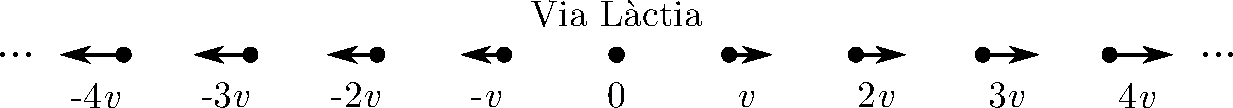
\includegraphics[width=0.8\textwidth]{./images/9-gal-no-centre}
	\caption{Il·lustració del repòs relatiu de la Via Làctia a l'Univers, que dóna la sensació que aquesta sigui el centre de l'Univers}
\label{fig:gal-no-centre}
\end{figure}

\subsubsection*{L'edat de l'Univers}
L'edat de la Terra, determinada a través de l'abundància relativa d'elements radioactius a la seva escorça és de $\approx \SI{4.5}{\giga\year}$. L'edat del sistema solar, estimada mitjançant l'abundància de \ch{^{87}Rb} relativa a la de \ch{^{87}Sr} en meteorits (\ch{^{87}Rb -> ^{87}Sr}, $\tau_{1/2} = \SI{4.99 e10}{\year}$) ve a ser aproximadament $\SIrange[range-units = repeat]{4.5}{5.0}{\giga\year}$. L'edat de les roques lunars se situa entre $\SIrange[range-units = repeat]{4.5}{4.6}{\giga\year}$. L'edat dels cúmuls globulars (a l'halo de la Galàxia) es troba en l'interval $\SIrange[range-units = repeat]{11.5}{16}{\giga\year}$.

L'edat estimada de l'Univers, $t_{0}$ (és a dir, el temps transcorregut des de l'inici de la seva expansió), segons resultats extrets de les dades del satèl·lit WMAP és
\begin{align*}
	t_{0} \approx \SI{13.7}{\giga\year}
\end{align*}
Aquest resultat és compatible amb $H_{0}^{-1} \approx \SI{14}{\giga\year}$, tal com prediuen els models cosmològics en voga.

\subsubsection*{L'abundància relativa d'heli}
El nucli d'heli (\ch{^{4}_{2}He}) és el més abundant a l'Univers després del d'hidrogen (\ch{^{1}_{1}H}); aproximadament 75\% d'hidrogen i 25\% d'heli en massa.

La major part de l'heli no és d'origen estel·lar sinó còsmic, produït en els primers instants de l'expansió de l'Univers a partir dels protons i neutrons lliures existents en aquella època.

La cadena de reaccions nuclears conduents a l'heli és complicada, no obstant el procés més significatiu és el següent:
\begin{align*}
\begin{cases}
	\ch{$p$ + $m$ -> D + $\gamma$} \\
	\ch{D + D -> ^{3}He + $n$ -> ^{3}H + $p$} \\
	\ch{^{3}He + D -> ^{4}He + $n$}
\end{cases}
\end{align*}
on $\ch{D} \equiv \ch{^{2}_{1}H}$ és el que anomenem deuteri o hidrogen pesant.

Aquest procés resulta efectiu un cop la temperatura del gas de fotons cau per sota de $T_{D} \approx \SI{8 e8}{\K}$, ja que quan $T > T_{D}$ el fas de fotons dissocia el deuteri (l'energia d'enllaç del deuteri és $B_{D} = m_{p} + m_{n} - m_{D} - \SI{1.71}{\MeV}$) de la següent manera:
\begin{align*}
	\ch{$\gamma$ + D -> $p$ + $n$}
\end{align*}

El fet que només el 25\% (en massa) dels nuclis siguin d'heli (i no pràcticament el 100\%) indica que l'Univers va passar per una fase de molt elevada temperatura caracteritzada per un gas de fotons amb temperatura superior a $T_{D}$.

La nucleosíntesi primordial (diferent de l'estel·lar) va finalitzar als 15 o 16 minuts d'iniciada l'expansió.

\subsubsection*{La radiació de fons de microones}
El gas de fotons es va anar refredant amb l'expansió de l'Univers:
\begin{align}
	T \propto \frac{1}{a}
\end{align}
on $a$ és el factor d'escala.

% FIXME: gamow@sec:bio
Com que el cas està en equilibri amb si mateix, ha de presentar una distribució de cos negre. L'existència d'aquest bany de radiació tèrmica va ser predita pels components de la nucleosíntesi primordial (George Gamow, Ralph Alpher, i Robert Herman) cap a finals dels anys 40 i descoberta fortuïtament pels astrofísics Arno Penxias i Robert Wilson al 1965.

La temperatura de la radiació de fons és avui de
\begin{align*}
	T_{0} \approx \SI{2.726}{\K}
\end{align*}
i, llevat de desviacions molt lleugeres, efectivament posseeix espectre de Planck (de cos negre).

Aquestes desviacions no són superiors a la centmil·lèsima part:
\begin{align*}
	\ev{\frac{\Delta T}{T_{0}}} \approx \num{e-5}
\end{align*}
Sense aquestes petites desviacions respecte al valor mitjà, $T_{0}$, l'existència de les galàxies no es podria entendre dins del model cosmològic estàndard (el més amplament acceptat).

Durant, aproximadament, els primers 380 mil anys de l'inici de l'expansió, la matèria (protons, electrons, i nuclis d'hidrogen, principalment) interaccionava amb la radiació (fotons) fonamentalment mitjançant
\begin{align*}
	\ch{$p$ + $e^{-}$ <-> H + $\gamma$}
\end{align*}
tot mantenint l'equilibri tèrmic entre matèria i radiació. Quan la temperatura va descendir per sota de $\approx \SI{3000}{\K}$, aquesta reacció ja no va ser efectiva per mantenir l'equilibri i els fotons es van poder propagar lliurement. Aquests fotons constitueixen la radiació de fons de microones (figura \ref{fig:dispersio-cmbr}).
\begin{figure}[h]
	\centering
	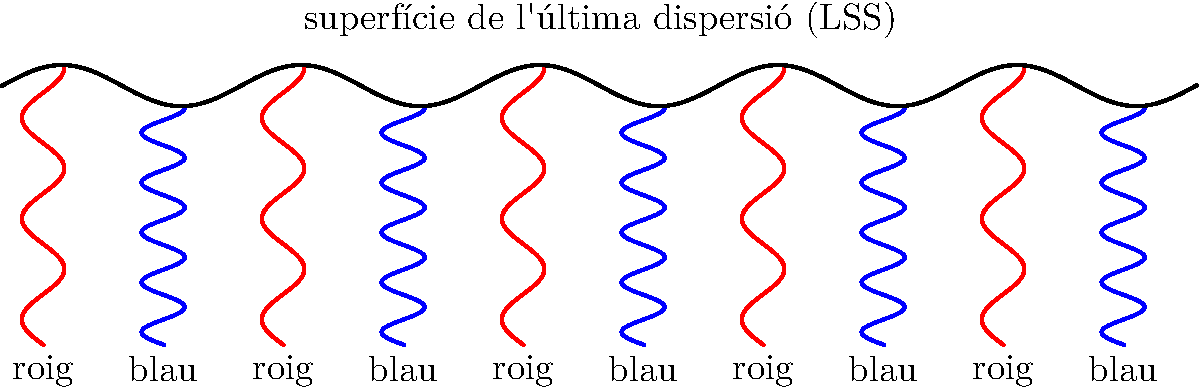
\includegraphics[width=0.85\textwidth]{./images/9-dispersio-cmbr}
	\caption{Diagrama simplificat de la superfície de l'última dispersió}
	\label{fig:dispersio-cmbr}
\end{figure}

%-----------------------------------------------------------------
\subsection{El model cosmològic estàndard}
\subsubsection*{El principi cosmològic}
D'igual manera que la Terra no ocupa una posició especial al sistema solar, ni aquest a la Galàxia, ni aquesta dins del nostre Grup Local, podem donar un pas més i formular la següent hipòtesi:
\begin{quote}
	\textit{«A una escala prou gran, l'aspecte que l'Univers presenta és independent del punt d'observació.»}
\end{quote}

Com podem veure a la figura \ref{fig:principi-cosmologic}, al petit cercle $A$ entorn l'observador $O$, la distribució de galàxies no és representativa de la densitat de galàxies a gran escala. Sí, en canvi, al cercle $B$.

Aquesta hipòtesi, a la pràctica, no és verificable (i podria no ser correcta) ja que avui només podem observar l'Univers des de la nostra galàxia.

El principi cosmològic no afirma que l'Univers sigui homogeni i isòtrop. Aquesta afirmació segueix d'advertir que és isòtrop\footnote{Cal notar que si un espai presenta isotropia en torn a cada punt, llavors és també homogeni.} en torn a la nostra galàxia (com l'observació mostra, específicament l'alt grau d'isotropia, $\sim \num{e-5}$, de la radiació de fons de microones), i d'aplicar el principi cosmològic.

Aquest principi comporta una gran simplificació a l'hora d'estudiar l'Univers des del punt de vista matemàtic.
\begin{figure}[h]
	\centering
	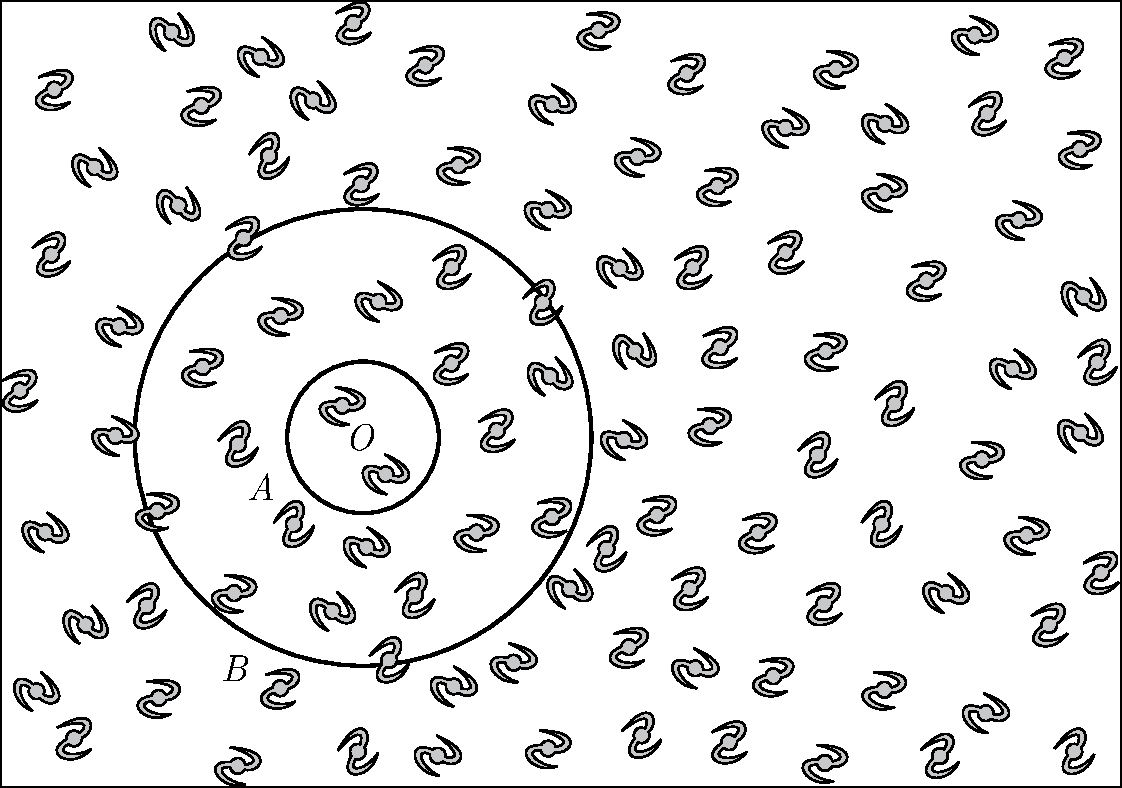
\includegraphics[width=0.7\textwidth]{./images/9-principi-cosmologic}
	\caption{El principi cosmològic. Per a l'observador ($O$) el cercle petit ($A$) no representa una distribució uniforme a gran escala. Al cercle gran ($B$) aquesta distribució ja és uniforme en mitjana}
	\label{fig:principi-cosmologic}
\end{figure}

\subsubsection*{Geometria de l'Univers: factor d'escala}
Si l'Univers és efectivament isòtrop (a gran escala) en torn a la Galàxia i acceptem el principi cosmològic, la distància entre si, de l'espai--temps ve donada per l'element de línia
\begin{align}\label{eq:flrw-metric}
	\dd{s^{2}} = - c^{2} \dd{t^{2}} + a^{2}(t) \qty{\frac{\dd{r^{2}}}{1 - kr^{2}} + r^{2}\dd{\theta^{2}} + \sin^{2} \theta \dd{\varphi^{2}}}
\end{align}
de la mètrica de Friedmann--Lemaître--Robertson--Walker. A aquesta mètrica, $a(t)$ és el \textit{factor d'escala}, una funció exclusiva del temps $t$. La constant $k$ és \textit{l'índex de curvatura espacial}:
\begin{align}
	k =
	\begin{cases}
		+ 1 & \text{esfera} \\
		\phantom{+} 0 & \text{pla} \\
		- 1 & \text{hiperboloide} \\
	\end{cases}
\end{align}

L'espai--temps de FLRW admet ser descompost en temps + espai tridimensional (aquest representat a la figura \ref{fig:time-space} per una superfície de només dues dimensions). Els observadors ($O_{A}, O_{B}, \dots$) es desplacen amb l'expansió de l'Univers sense velocitat pròpia (o velocitat peculiar). Les seves coordenades espacials ($r, \theta, \varphi$) són les mateixes en cada superfície espacial, les quals són homogènies i isòtropes.
\begin{figure}[h]
	\centering
	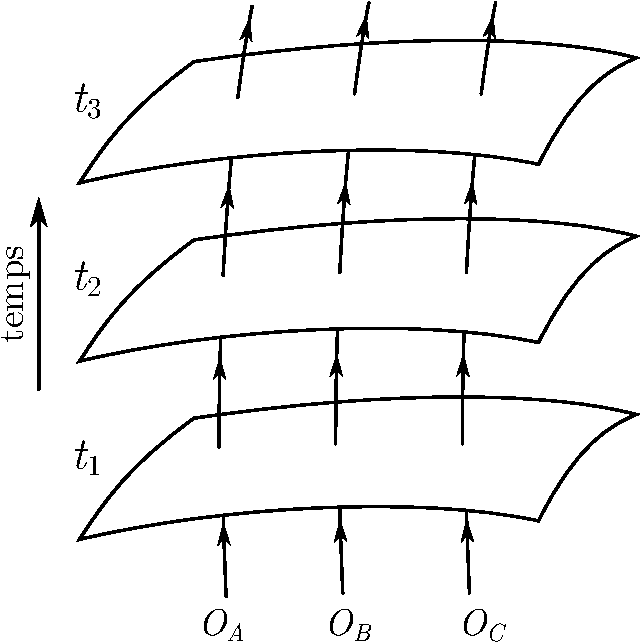
\includegraphics[width=0.45\textwidth]{./images/9-time-space}
	\caption{Il·lustració simplificada d'una hipersuperfície d'espai--temps}
	\label{fig:time-space}
\end{figure}

El factor d'escala ens indica l'augment o disminució de la distància espacial entre cada parell d'observadors en passar d'una a una altra hipersuperfície:
\begin{align}
	\frac{a(t_{1})}{a(t_{2})} = \frac{D_{AB}(t_{1})}{D_{AB}(t_{2})}
\end{align}

Així doncs, si la distància a l'instant $t$ a una galàxia era $r(t)$, avui dia (instant $t_{0}$) la distància, prescindint del moviment peculiar serà
\begin{align}
	r_{0} = \frac{a(t_{0})}{a(t)} r(t)
\end{align}

En sistemes no lligats gravitacionalment, les longituds augmenten en proporció a l'expansió de l'Univers, és a dir, al factor d'escala $a(t)$. Per tant, si la longitud d'ona d'un fotó en un instant $t < t_{0}$ és $\lambda$, la seva longitud d'ona serà
\begin{align}
	\lambda_{0} = \frac{a{0}}{a} \lambda
\end{align}
Com que el redshift, $z$, es defineix com $z = \Delta \lambda / \lambda$, es veu que
\begin{align}\label{eq:redshift-a}
	1 + z = \frac{a_{0}}{a}
\end{align}

Llavors, el redshift d'una galàxia llunyana ens indica quant s'ha expandit l'Univers des de l'instant en què aquesta galàxia va emetre la llum que avui arriba al nostre detector i l'instant actual.

Així, la llum d'una galàxia de redshift $z = 1$ va ser emesa quan el factor d'escala era només la meitat que el d'avui; és a dir, aquesta galàxia estava de nosaltres a la meitat de la distància en què es troba avui.

Per a $0 < z \ll 1$, l'equació \eqref{eq:redshift-a} és quasi idèntica a la llei de Hubble, \eqref{eq:hubble-law}. Efectivament, per a $z$ petit el canvi en $a(t)$ serà proporcional al temps $t$ que la llum porta viatjant. Però $t = r/c$, llavors $z \propto r/c$, on $r$ és la distància a la galàxia que va emetre la llum. La constant de proporcionalitat ha de tenir unitats d'invers de temps, llavors ha de ser $H_{0}$. Així es recupera
\begin{align}
	z = \frac{H_{0}}{c} r \tag{\ref{eq:hubble-law} revisitada}
\end{align}

\subsubsection*{Equacions bàsiques del model cosmològic estàndard}
Aquest model s'assenta en varies pressuposicions:
\begin{itemize}
	\item L'Univers és homogeni i isòtrop $\Rightarrow$ descrit per la mètrica de FLRW a grans escales.
	\item La validesa de la teoria de gravitació d'Albert Einstein (teoria general de la relativitat).
	\item El contingut de l'Univers a gran escala es pot modelar per un o varis fluids perfectes (fluids que no presenten dissipació, és a dir, que flueixen adiabàticament).
\end{itemize}

Les equacions bàsiques del model són la de Friedmann \eqref{eq:friedmann} i la de l'acceleració \eqref{eq:acceleration}:
\begin{align}\label{eq:friedmann}
	3 H^{2} + 3 \frac{k}{a^{2}} = 8\pi G \rho
\end{align}
\begin{align}\label{eq:acceleration}
	3 \frac{\ddot{a}}{a} = -4\pi G (\rho + 3P)
\end{align}
on $\rho$ és la densitat d'energia dels fluids (e.g., matèria i/o radiació), $P$ és la pressió dels fluids, $G = \SI{6.67 e-8}{\dyn \per\square\cm \per\square\g}$ és la constant de gravitació, i $H \equiv \dot{a}/a$ és el factor de Hubble.

De les equacions \eqref{eq:friedmann} i \eqref{eq:acceleration} es pot deduir l'equació de la conservació de l'energia:
\begin{align}\label{eq:energy-cons1}
	\dot{\rho} + 3H (\rho + P) = 0
\end{align}
però és lleugerament més immediat arribar a ella a partir de l'equació de Gibbs $T \dd{S} = \dd{E} + P \dd{V}$ per a processos isentròpics, $\dd{E} + P \dd{V} = 0$. Aquí, $E = \rho a^{3}$ i $V = a^{3}$, llavors
\begin{align}\label{eq:energy-cons2}
	\dd{(\rho a^{3})} + P \dd{a^{3}} = 0
\end{align}
equació equivalent a \eqref{eq:energy-cons1}.

La deducció de les equacions \eqref{eq:friedmann} i \eqref{eq:acceleration} està més enllà del nivell d'aquest curs i no ho farem aquí. No obstant això, és possible una deducció un tant \textit{ad hoc} a partir de la teoria de Newton de la gravitació.

Sabem que una partícula submergida en una distribució esfèrica i homogènia de matèria no experimenta força gravitatòria alguna per la matèria més allunyada que la del centre d'aquesta distribució. Llavors, el mòdul de la força a la qual aquesta partícula està sotmesa és $F = G \dfrac{M m}{r^{2}}$; de forma que la seva energia potencial és $ V = -G \dfrac{M m}{r} = - \dfrac{4\pi}{3} G M \rho r^{2}$, i la seva energia cinètica és $T = \dfrac{1}{2} m \dot{r}^{2}$. Passant de coordenades físiques, $\va{r}$, a coordenades comòbils (il·lustrat a la figura \ref{fig:comobils}), $\va{x}$ (fent el canvi $\va{r} = a(t) \va{x}$), tenim
\begin{align*}
	U = \frac{1}{2} m \dot{a}^{2} x^{2} - \frac{4\pi}{3} G \rho a^{2} x^{2} m
\end{align*}
\begin{figure}[h]
	\centering
	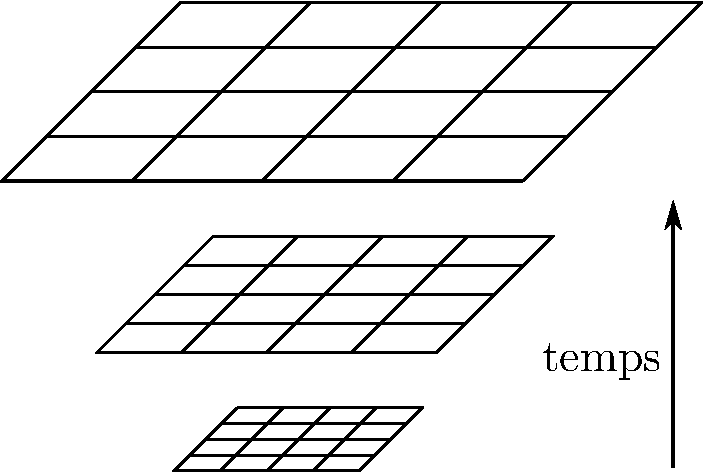
\includegraphics[width=0.4\textwidth]{./images/9-comobils}
	\caption{El sistema de coordenades comòbils canvia juntament amb l'expansió, de manera que els objectes romanen sempre a les mateixes coordenades}
	\label{fig:comobils}
\end{figure}

Multiplicant per $2/(m a^{2} x^{2})$ i reordenant s'obté l'equació de Friedmann:
\begin{align}
	3 \qty(\frac{\dot{a}}{a})^{2} + 3 \frac{k}{a^{2}} = 8\pi G \rho \tag{\ref{eq:friedmann} revisitada}
\end{align}
identificant $k = -2U/(mx^{2})$. El terme $k$ és constant, ja que ni $U$, ni $m$, ni la posició $\va{x}$ de la partícula (suposant que no té velocitat peculiar, només la de l'expansió de l'Univers) depenen del temps.

Es pot comprovar que l'equació de l'acceleració \eqref{eq:acceleration} s'obté de combinar les equacions \eqref{eq:friedmann} i \eqref{eq:energy-cons1}. Tanmateix, es pot veure que:
\begin{enumerate}[(i)]
	\item A partir de l'equació de la conservació de l'energia, \eqref{eq:energy-cons1}, i l'equació d'estat de la radiació, $P = \rho/3$, s'obté que la densitat d'energia de la radiació obeeix $\rho_{rad} \propto a^{-4}$.
	\item A partir de l'equació de la conservació de l'energia, \eqref{eq:energy-cons1}, i l'equació d'estat de la matèria freda (no relativista), $P = 0$, s'obté que la densitat d'energia de la matèria obeeix $\rho_{mat} \propto a^{-}$.
	\item Sabent que la densitat d'energia de la radiació depèn de la temperatura com $\rho_{rad} \propto T_{rad}^{4}$, s'obté que $T_{rad} \propto 1/\alpha$.
\end{enumerate}

La dependència del factor d'escala amb el temps ve expressada gràficament a la figura \ref{fig:factor-escala}. Aquesta dependència s'obté analíticament combinant l'equació de Friedmann \eqref{eq:friedmann} amb $\rho = \rho_{0} (a_{0}/a)^{3}$, en el cas que l'energia que emplena l'Univers sigui matèria no relativista (pressió nul·la), o amb $\rho = \rho_{0} (a_{0}/a)^{4}$ si l'energia és relativista (radiació; $P = \rho/3$). Per a $k = 0$ s'obté
\begin{align}
 \begin{cases}
	a(t) \propto t^{1/2} & \text{(radiació)} \\
	a(t) \propto t^{2/3} & \text{(matèria no relativista)}
 \end{cases}
\end{align}
Les solucions per a $k \neq 0$ no es mostren aquí.

\begin{figure}[h]
	\centering
	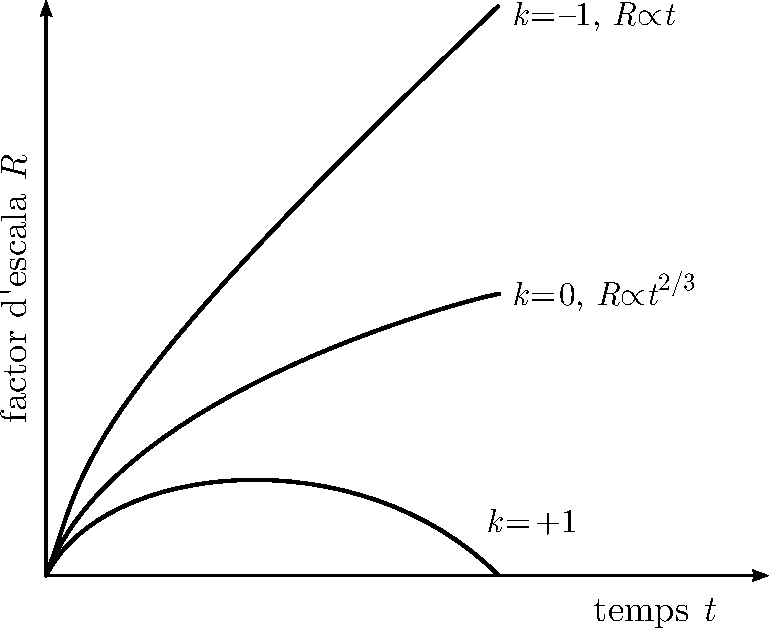
\includegraphics[width=0.6\textwidth]{./images/9-factor-escala}
	\caption{Esbós de l'evolució del factor d'escala amb el temps, qualitativament vàlid tant si la matèria és relativista com si no}
	\label{fig:factor-escala}
\end{figure}

\begin{example}
	Volem demostrar que si l'Univers de FLRW pla ($k = 0$) està dominat per la matèria no relativista ($P = 0$), el factor d'escala obeeix $a(t) \propto t^{2/3}$.

	Efectivament, de l'equació de la conservació de l'energia, suposada l'expansió adiabàtica, \eqref{eq:energy-cons2} se segueix $\rho a^{3} = cte$ si $P = 0$. Combinant aquesta equació amb l'equació de Friedmann \eqref{eq:friedmann} per a $k = 0$, s'obté que $a \dot{a}^{2} = A^{2}$, on $A^{2} \equiv \dfrac{8\pi G}{3} \rho a^{3} = cte$. Llavors
	\begin{align*}
		A \int_{0}^{t} \dd{t} = \int_{0}^{a} a^{1/2} \dd{a} \Rightarrow t = \frac{2}{3A} a^{3/2}
	\end{align*}
	és a dir,
	\begin{align*}
		a(t) = \qty(4\pi G \rho_{0} a_{0}^{3})^{2/3} t^{2/3}
	\end{align*}
\end{example}

Cal advertir que podem expressar el temps $t = 2a^{3/2}/(3A)$ com
\begin{align}
	t = \frac{2}{3} \frac{a^{3/2}}{\sqrt{\dfrac{8\pi G}{3} \rho_{0} a_{0}^{3}}} \equiv \frac{2}{3 H_{0}} \qty(\frac{a}{a_{0}})^{3/2}
\end{align}
de manera que, en aquest simple model, l'edat de l'Univers vindrà donada per $t_{0} = 2/(3 H_{0})$. Com que $H_{0} \approx \SI{70}{\km \per\s \per\mega\parsec}$, l'edat predita ($\approx \SI{9.3}{\giga\year}$) és inferior a la dels cúmuls globulars.

La discrepància es resol si s'admet que l'energia de pressió negativa (ja sigui l'energia del buit quàntic o, més en general, energia fosca) contribueix actualment de forma important a l'expansió de l'Univers.

Com la figura \ref{fig:factor-escala} mostra, si a l'energia de l'Univers contribueix només radiació i/o matèria no relativista, aquest s'expandirà sempre si $k = 0$ o si $k = -1$, i es contraurà ($\dot{a} < 0$) després d'una expansió màxima si $k = 1$. En aquest últim cas, arribarà un instant en què el factor d'escala s'anul·larà. Es pot demostrar que per a un Univers dominat per la matèria ($P = 0$) i de seccions espacials esfèriques ($k = 1$), el màxim valor del factor d'escala és
\begin{align*}
	a_{\max} = \frac{8\pi G}{3} \rho_{0} a_{0}^{3}
\end{align*}

Mesures de l'expansió de l'Univers suggereixen que aquest no s'expandeix a un ritme constant (és a dir $H(t) \neq cte$). La magnitud adimensional que quantifica si l'expansió s'accelera o frena és el \textit{paràmetre de desacceleració}
\begin{align}
	q = - \frac{\ddot{a}}{a H^{2}}
\end{align}
Mesures recents semblen indicar que el seu valor avui dia és $q_{0} \approx - 0.5$; és a dir, l'Univers està accelerant la seva expansió ($\ddot{a} > 0$).

Es pot demostrar que si $k = 0$ (seccions espacials planes), $q = 1$ si l'energia dominant és la radiació, i $q = 1/2$ si és la matèria no relativista.

Abans mencionàvem que les densitats d'energia de la matèria i la radiació varien amb el factor d'escala d'acord a $\rho_{m} = \rho_{m0} (a_{0}/a)^{3}$ i $\rho_{r} = \rho_{r0} (a_{0}/a)^{4}$, respectivament. Com la figura \ref{fig:mat-rad-factor-escala} mostra, a partir de cert valor d'escala, $a_{eq}$, la matèria domina sobre la radiació ($\rho_{m} > \rho_{r}$), mentre que per a $a < a_{eq}$ la radiació domina sobre la matèria ($\rho_{r} > \rho_{m}$).

Mesures observacionals mostren que $\rho_{m0}/\rho_{r0} \approx \num{2 e4}$. Es conclou immediatament que el redshift pel qual $\rho_{m} = \rho_{r}$ és, aproximadament, $z_{eq} \approx \num{2 e4}$.
\begin{figure}[H]
	\centering
	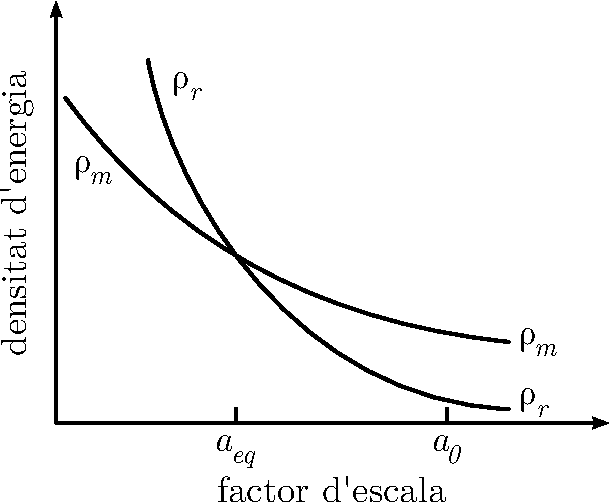
\includegraphics[width=0.45\textwidth]{./images/9-mat-rad-factor-escala}
	\caption{Esbós de l'evolució de les densitats d'energia de la matèria freda i la radiació amb el factor d'escala. Aquí, $a_{eq}$ és el valor del factor d'escala per al qual es dóna la igualtat matèria--radiació}
	\label{fig:mat-rad-factor-escala}
\end{figure}

%-----------------------------------------------------------------
\subsection{Formació d'estructures còsmiques}
Després de l'època de la recombinació ($z_{rec} \approx 1089$) els fotons van quedar desacoblats dels barions (protons i neutrons) i aquests, lliures de la pressió de la radiació, van poder caure sense oposició als pous de potencial gravitatori creats prèviament per la matèria fosca (fonamentalment WIMPs).

Una regió on la densitat de matèria és lleugerament superior al valor mitjà disminuirà el seu ritme d'expansió i se separarà de la matèria que la rodeja.

Si el contrast de densitats, $\delta{m} = \delta \rho_{m} / \bar{\rho}_{m} = (\rho_{m} - \bar{\rho}_{m}) / \bar{\rho}_{m}$ és suficientment gran, aquesta regió cessarà d'expandir-se i col·lapsarà, arribant amb el temps a formar alguna mena d'estructura còsmica (un cúmul globular, una galàxia, un grup o un cúmul de galàxies).

El temps invertit en el col·lapse és, aproximadament
\begin{align}
	\Delta t_{col} \approx \frac{10^{6}}{\sqrt{\Omega_{0}} h} \frac{10^{3}}{z_{rec}} \delta^{-3}_{m}
\end{align}
on $\Omega_{0} \approx 1$, i $h \approx 0.7$. Així les pertorbacions de densitat més intenses (major $\delta_{m}$) inverteixen menys temps en col·lapsar.

Com la figura \ref{fig:contrast-densitats-wimp} mostra, el contrast de densitats de la matèria no bariònica (WIMPs) comença a crèixer apreciablement a partir de l'època de la igualtat matèria--radiació ($a_{eq}$).

El contrast de densitats dels barions roman constant fins just després del desacoblament matèria--radiació. A partir d'aquí augmenta ràpidament (ja que els barions són atrets gravitacionalment per les concentracions de matèria fosca) de forma que després d'un cert temps després de $a_{dec}$, ambdós contrasts de densitats venen a ser aproximadament iguals
\begin{align*}
	\delta_{bar} \approx \delta_{dm}
\end{align*}
i els dos tipus de pertorbacions creixen juntes.
\begin{figure}[h]
	\centering
	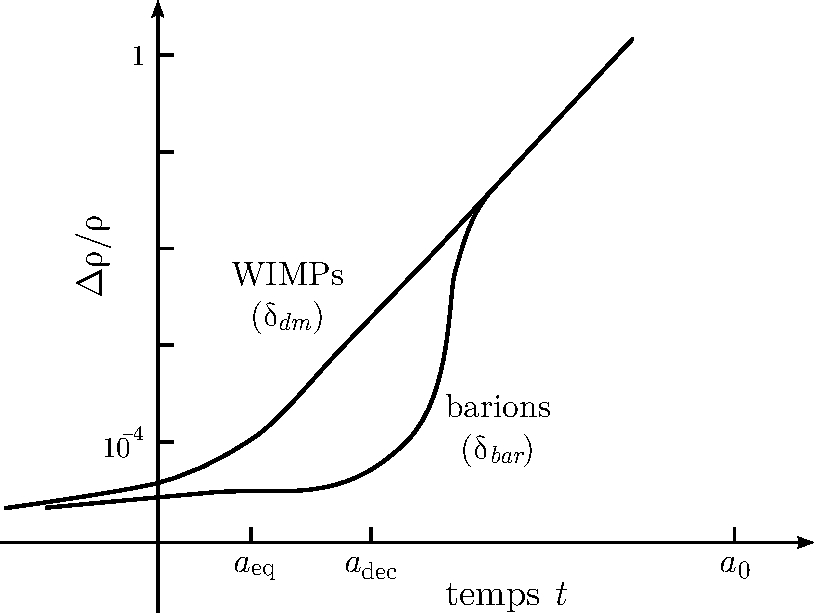
\includegraphics[width=0.6\textwidth]{./images/9-contrast-densitats-wimp}
	\caption{Evolució del contrast de densitats de la matèria fosca (WIMPs) i dels barions}
	\label{fig:contrast-densitats-wimp}
\end{figure}

Cal notar que les pertorbacions de matèria (tant bariònica com de matèria fosca) creixeran només si la gravitació dins la pertorbació és més intensa que la força interna de pressió és oposada al col·lapse. Això implica que perquè es produeixi el col·lapse (i per tant, la pertorbació termina per formar alguna estructura còsmica) és necessari que la mida, $\lambda$, de la pertorbació sigui major que la distància, $\lambda_{J}$, recorreguda pel so durant el temps invertit en un col·lapse lliure (suposant que la pressió de s'oposa al col·lapse):
\begin{align*}
	\lambda \geq \lambda_{J}
\end{align*}
on $\lambda_{J} = c_{s} \tau_{ff}$, sent $c_{s}$ la velocitat del so en un fluid còsmic, i $\tau_{ff} \approx \sqrt{\pi / (G \rho)}$ el temps invertit en un col·lapse lliure.

La distància $\lambda_{J}$ es coneix com \textit{longitude Jeans}, i la massa corresponent (suposant un cos esfèric) es coneix com \textit{massa de Jeans}:
\begin{align}
	M_{J} = \frac{4pi}{3} \lambda_{J}^{3} \rho = \frac{4\pi}{3} c_{s}^{3} \rho \qty(\frac{\pi}{G \rho})^{3/2}
\end{align}

Per tant, si $M > M_{J}$ es produirà el col·lapse i la pertorbació arribarà a formar un cúmul globular, una galàxia, o un cúmul de galàxies. En canvi si $M < M_{J}$, la pertorbació oscil·larà en torn a un valor inferior a $M_{J}$ i no es produirà estructura còsmica alguna (figura \ref{fig:no-structure}).
\begin{figure}[h]
	\centering
	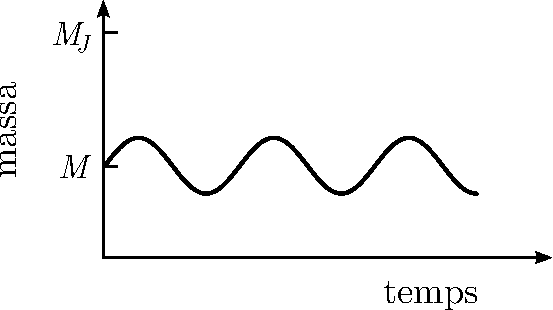
\includegraphics[width=0.41\textwidth]{./images/9-no-structure}
	\caption{Oscil·lació de $M$ en torn a un valor inferior a $M_{J}$, impedint la formació d'estructures còsmiques}
	\label{fig:no-structure}
\end{figure}

Al model cosmològic estàndard
\begin{align*}
	M_{J} \approx \frac{10^{6}}{\Omega_{0} h^{3}} \si{\Msun}
\end{align*}
després de la recombinació matèria--radiació ($z_{rec} \approx 1089$). Aquest valor de $M_{J}$ és de l'ordre de la massa dels cúmuls globulars (possiblement les primeres estructures en formar-se i, per tant, les més antigues.

La figura \ref{fig:jeans-mass} mostra la dependència de la massa de Jeans amb respecte al factor d'escala.
\begin{figure}[h]
	\centering
	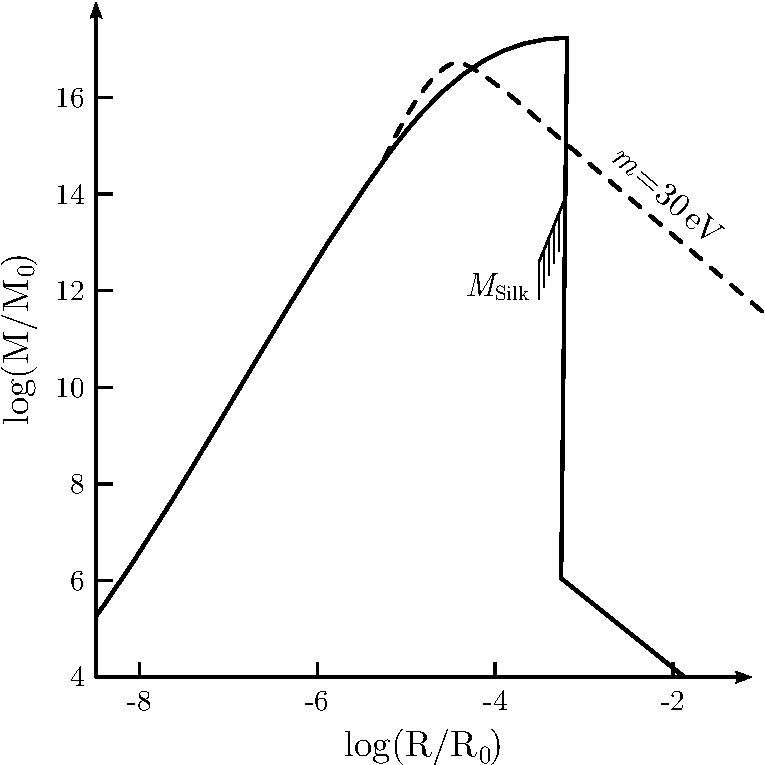
\includegraphics[width=0.55\textwidth]{./images/9-jeans-mass}
	\caption{Massa de Jeans front al factor d'escala}
	\label{fig:jeans-mass}
\end{figure}

La forta caiguda de $M_{J}$ per a $a/a_{0} \approx \num{e-3}$ és degut al súbit descens de la velocitat del so en passar de $z \gtrsim z_{rec}$ a $z \lesssim z_{rec}$. A partir d'aquest moment, $M_{J}$ decreix com $M_{J} \propto a^{-3/2}$. Això facilita molt el col·lapse de les pertorbacions (fluctuacions) de la matèria.

L'evolució del contrast de densitats per matèria no relativista ($P = 0$) depèn de la mida, $\lambda$, de la fluctuació i dels valors de $\Omega_{0}$ i $H_{0}$ tal com mostra la figura \ref{fig:contrast-densitats-mat} (on $h = H_{0}/100 \approx 0.7$, $\Omega_{0} \approx 1$). Per a escales suficientment grans, es compleix
\begin{align}
	\delta_{m} = \frac{\delta\rho_{m}}{\rho_{m}} \propto \lambda^{-2} \propto M^{-2/3}
\end{align}
\begin{figure}[h]
	\centering
	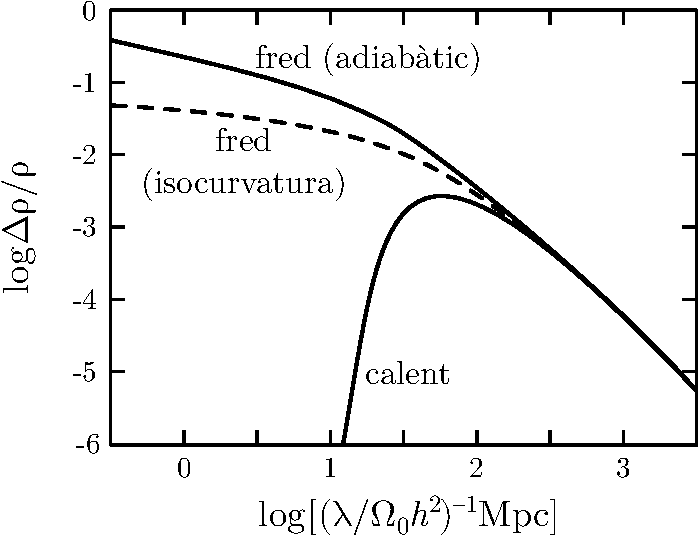
\includegraphics[width=0.5\textwidth]{./images/9-contrast-densitats-mat}
	\caption{Contrast de densitats per a la matèria freda front a l'escala de la pertorbació en un instant genèric després de la igualtat matèria--radiació}
	\label{fig:contrast-densitats-mat}
\end{figure}

\subsubsection*{Formació de galàxies i cúmuls}
L'alt grau d'isotropia de la radiació de fons de microones ens indica que les galàxies no es van formar a partir de la inestabilitat gravitacional de matèria purament bariònica (de ser així, $\ev{\Delta T/T_{0}}$ hauria de ser molt major que $\num{e-5}$).

Això ens porta a concloure que les galàxies es van formar per inestabilitat gravitacional de matèria fosca no bariònica (WIMPs) i matèria bariònica (la primera en major proporció, unes cinc vegades més, que la segona).

L'escenari més acceptat avui sosté que, degut a inestabilitats gravitacionals, la matèria fosca no bariònica s'hauria condensat (parcialment, al menys) en grumolls (a petita escala, menys que el radi de l'horitzó, $c H^{-1}$) els quals s'agregarien entre si per formar els halos de les galàxies. Després del desacoblament matèria--radiació, $z_{rec} \approx 1089$, la matèria bariònica cauria al centre dels halos (pou de potencial gravitatori) donant lloc a la part visible de les galàxies. Posteriorment, mitjançant atracció gravitatòria de les unes amb les altres, les galàxies s'aproparien entre si formant galàxies, cúmuls i supercúmuls.

En la fase inicial (lineal) el contrast de densitats de la matèria freda (no relativista, $P = 0$)
\begin{align*}
	\delta_{m} = \frac{\rho_{m} - \bar{\rho}_{m}}{\bar{\rho}_{m}}
\end{align*}
obeeix l'equació diferencial
\begin{align}\label{eq:dif-contrast}
	\ddot{\delta}_{m} + 2\frac{\dot{a}}{a} \delta_{m} - 4\pi G \rho_{m} \delta_{m} = 0
\end{align}

Es pot deduir que per a un Univers de seccions espacials planes ($k = 0$) dominat per la matèria, $a(t) \propto t^{2/3}$, les solucions a l'equació \eqref{eq:dif-contrast} són $\delta_{m} \propto t^{2/3}$ (mode creixent) i $\delta_{m} \propto t^{-1}$ (mode decreixent). En aquest escenari, el mode creixent és el responsable de la formació d'estructures còsmiques.

L'espectre de fluctuacions (pertorbacions) a gran escala i la radiació de fons de microones compatible amb un univers dominat avui dia per la matèria no relativista (bariònica més no bariònica) i energia fosca de pressió negativa (possiblement l'energia del buit quàntic) de seccions espacials planes ($k = 0$). Més concretament,
\begin{align*}
	\Omega_{m} = \Omega_{dm} + \Omega_{b} \approx 0.28 \qc \Omega_{\Lambda} \approx 0.72 \qc \Omega_{k} \approx 0
\end{align*}
on $\displaystyle \Omega_{dm} = \frac{8\pi G \rho_{m0}}{3 H_{0}^{2}}$, $\displaystyle \Omega_{b} = \frac{8\pi G \rho_{b0}}{3 H_{0}^{2}}$, $\displaystyle \Omega_{\Lambda} = \frac{8\pi G \rho_{\Lambda}}{3 H_{0}^{2}}$, $\displaystyle \Omega_{k} = \frac{-k}{a_{0}^{2} H_{0}^{2}}$; amb $H_{0} \approx \SI{70.1}{\km \per\s \per\mega\parsec}$.

Per descriure l'agrupament de galàxies se sol utilitzar la funció de correlació $\xi(r)$, definida com
\begin{align}
	\dd{P} = (\bar{n})^{2} \qty[ 1 + \xi(\va{r}_{2} - \va{r}_{1})] \dd[3]{\va{r}_{1}} \dd[3]{\va{r}_{2}}
\end{align}
on $\dd{P}$ és la probabilitat conjunt de trobar una galàxia a l'interval $[\va{r}_{1}, \va{r}_{1} + \dd{\va{r}_{1}}]$ i una altra a l'interval $[\va{r}_{2}, \va{r}_{2} + \dd{\va{r}_{2}}]$; $\bar{n}$ és el nombre mitjà de galàxies en la unitat de volum.

Si l'Univers és homogeni i isòtrop, llavors $\norm{\va{r}_{2} - \va{r}_{1}} = r \Rightarrow \xi(\va{r}_{2} - \va{r}_{1}) = \xi(r)$.

Així doncs, $\xi(r)$ ens quantifica l'excés de probabilitat de trobar una galàxia a la distància $r$ d'una altra qualsevol triada a l'atzar.

L'observació mostra que els cúmuls de galàxies semblen ser més densament agrupats que les galàxies entre si:
\begin{align*}
	\xi(r)_{gal} \sim \qty(\frac{r}{5 h^{-1}\,\si{\mega\parsec}})^{-1.8} \qc \xi(r)_{cum} \sim \qty(\frac{r}{2.5 h^{-1}\,\si{\mega\parsec}})^{-1.8}
\end{align*}

Les simulacions per ordinador (figura \ref{fig:cluster-evolution-cdm}) concorden en línies generals amb les expressions de $\xi(r)$. La figura \ref{fig:power-spectrum} mostra \textit{l'espectre de potència de la matèria}
\begin{align}
	P(k) = \ev{\abs{\delta_{k}}^{2}}
\end{align}
en funció del nombre d'ona $\displaystyle k = \frac{2\pi}{\lambda a}$.

\begin{figure}[H]
	\centering
	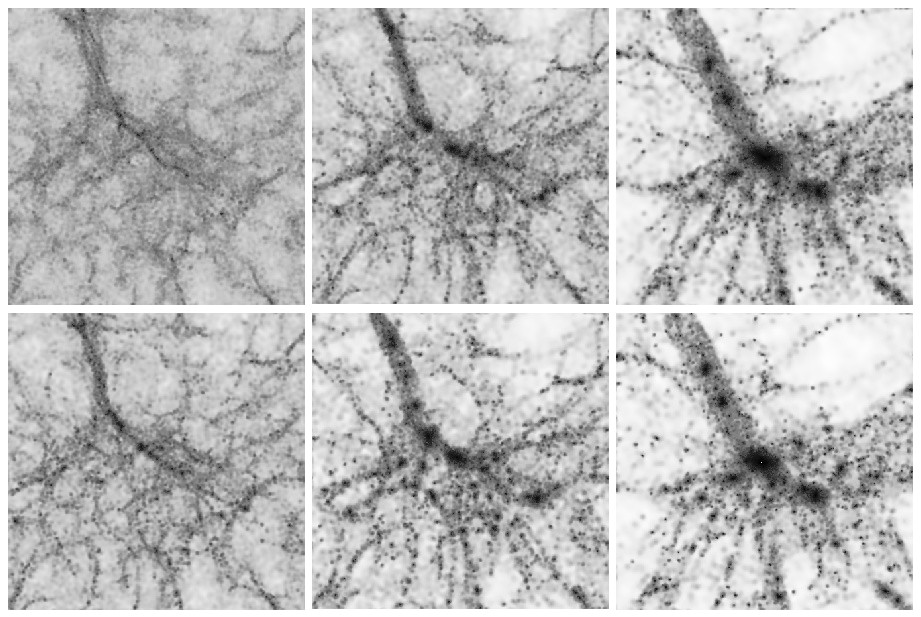
\includegraphics[width=0.7\textwidth]{./images/9-cluster-evolution-cdm}
	\caption{Evolució del mateix cúmul als models $\tau$CDM (imatges superiors) i $\Lambda$CDM (imatges inferiors), per a redshifts $z = 2$ (esquerra), $z = 1$ (centre), $z = 0$ (dreta).}
	\label{fig:cluster-evolution-cdm}
\end{figure}

Aquí $\delta_{k}$ depèn del factor d'escala i està relacionat amb el contrast de densitats de la matèria a través de la transformada de Fourier
\begin{align*}
	\delta(\va{r},a) \equiv \frac{\rho_{m}(\va{r},a) - \bar{\rho}_{m}(\va{r},a)}{\bar{\rho}_{m}(\va{r},a)} = \int \delta_{k}(a) \exp[i \va{k} \va{r}] \dd[3]{k}
\end{align*}
\begin{figure}[H]
	\centering
	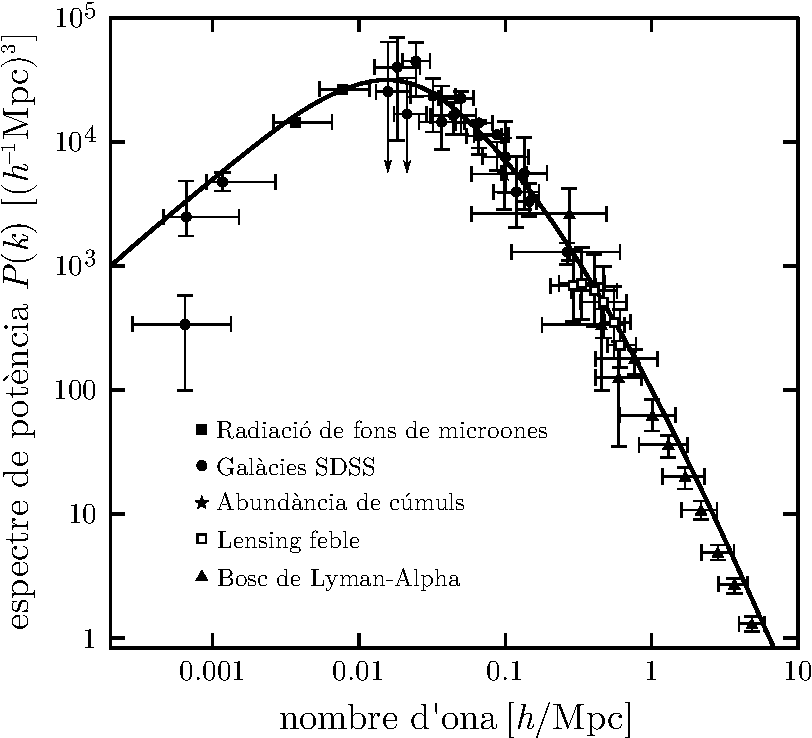
\includegraphics[width=0.6\textwidth]{./images/9-power-spectrum}
	\caption{L'espectre de potència $P(k)$ mesurat en funció del nombre d'ona $k$}
	\label{fig:power-spectrum}
\end{figure}

El comportament de la funció $P(k)$ depèn de l'escala (figura \ref{fig:power-spectrum}):
\begin{align}
	P(k) \propto
	\begin{cases}
		k & \text{per a } k \ll k_{eq} \; (a\lambda \gg c H_{eq}^{-1}) \\
		k^{-3} & \text{per a } k \gg k_{eq} \; (a\lambda \ll c H_{eq}^{-1})
	\end{cases}
\end{align}

Un cop les pertorbacions de densitat es fan més pronunciades ($\delta_{m}$ creix) i se separen del gas de partícules circumdant, el seu destí depèn de com d'eficaç sigui el procés de formació d'estrelles a la fase de col·lapse. En concret, la pertorbació acabarà formant una galàxia el·líptica si tot el gas bariònic (fonamentalment àtoms d'hidrogen i d'heli) dóna lloc a estrelles abans que la pertorbació acabi de col·lapsar. Si no fos així, es tindria una galàxia espiral (un disc sostingut per forces centrífugues i englobat en un cos el·lipsoidal).

Després de formades, les galàxies evolucionen mitjançant col·lisions amb altres galàxies i fagocitació. Moltes galàxies el·líptiques i lenticulars poden haver resultat de la unió de protogalàxies amb elevat contingut de gas.

La figura \ref{fig:galaxy-formation-z} mostra una estimació del ritme de formació de galàxies en termes del redshift, $z$, basada en estudis a diferents longituds d'ona (visible, infraroja, i submil·limètrica).
\begin{figure}[H]
	\centering
	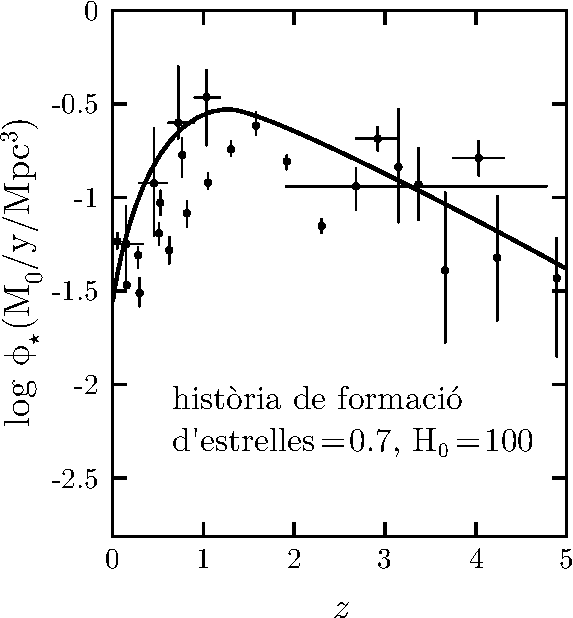
\includegraphics[width=0.45\textwidth]{./images/9-galaxy-formation-z}
	\caption{Ritme de formació de galàxies en funció del redshift}
	\label{fig:galaxy-formation-z}
\end{figure}

\subsubsection*{Contribució de les galàxies a la densitat de l'Univers}
Com ja hem vist anteriorment, la funció de Schechter \eqref{eq:schechter} ens dóna una estimació del nombre de galàxies, $\Phi (L) \dd{L}$, per $\si{\cubic\mega\parsec}$, amb lluminositat en l'interval $(L, L + \dd{t})$. Suposant que la relació massa--lluminositat de les estrelles en galàxies és $M/L = 5$, es troba que avui ($z = 0$) el valor amb què les galàxies contribueixen a la densitat de l'Univers és
\begin{align*}
	\rho_{gal} \approx \num{2 e-32} \qty(\frac{H_{0}}{50})^{2} \si{\g \per\cubic\cm}
\end{align*}
o, equivalentment,
\begin{align*}
	\Omega_{gal} = \frac{8 \pi G \rho_{gal}}{3 H_{0}^{2}} \approx 0.004
\end{align*}

Aquest valor és 10 vegades inferior a l'inferit de la nucleosíntesi primordial, i unes 70 vegades per sota de l'estimat per a la matèria total (bariònica i no bariònica, $\Omega_{m} = 0.28$). Així, només el 10\% dels barions es troben a les estrelles. A més, aproximadament només el 4.5\% de la matèria de l'Univers és bariònica.

La figura \ref{fig:densitat-univers} mostra la contribució relativa de galàxies de diferents masses a la densitat de l'Univers. Galàxies amb masses a l'interval $\SIrange{e10}{e12}{\Msun}$ proporcionen la major contribució. Fora d'aquest rang la contribució relativa decau fortament. La corba de la figura s'ha extrapolat cap a la dreta amb fi d'incloure cúmuls globulars aïllats.
\begin{figure}[h]
	\centering
	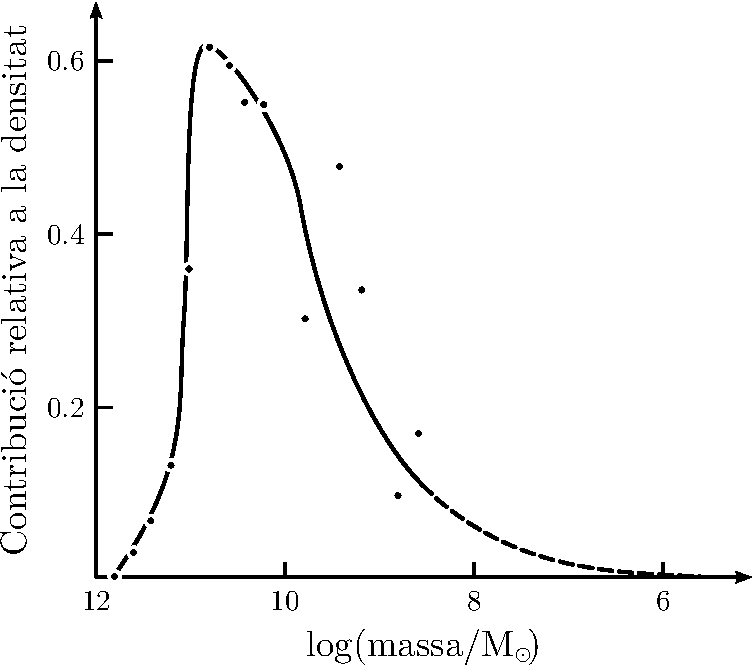
\includegraphics[width=0.55\textwidth]{./images/9-densitat-univers}
	\caption{Contribució relativa de galàxies de diferents masses a la densitat de l'Univers}
	\label{fig:densitat-univers}
\end{figure}

Als últims anys s'han portat a terme (i continuen en marxa) extenses exploracions del cel. Per això, avui es pot disposar de mapes de la distribució de galàxies en termes del redshift $z$, alhora que s'ha pogut obtenir una estimació fiable de $\Omega_{m}$ mitjançant l'anàlisi de les velocitats peculiars de les galàxies. Els resultats suggereixen que $\Omega_{m} = \num{0.3 \pm 0.2}$.

Com que $\Omega_{0} \approx 1$, s'infereix la presència d'una energia no lluminosa (fosca), i molt uniformement distribuïda que contribueix en un 70\%, aproximadament, a la densitat de l'Univers.

Aquests mapes revelen que les galàxies, es troben distribuïdes irregularment, no a l'atzar, agrupades en grups, cúmuls, supercúmuls. Aquests, a la vegada, estan disposats en una intricada xarxa de filaments i parets, enfilades per túnels (figura \ref{fig:mapa-redshift}). Així doncs, la distribució de galàxies a gran escala està estructurada en un ampli rang d'escales.

Aparentment, a certes escales, la distribució presenta estructura fractal. Si això s'estengués a les màximes escales accessibles, la distribució de galàxies no seria homogènia. No obstant això, s'ha trobat que el comportament fractal es limita a escales per sota de $\SI{200}{\per\planck \mega\parsec}$.
\begin{figure}[h]
	\centering
	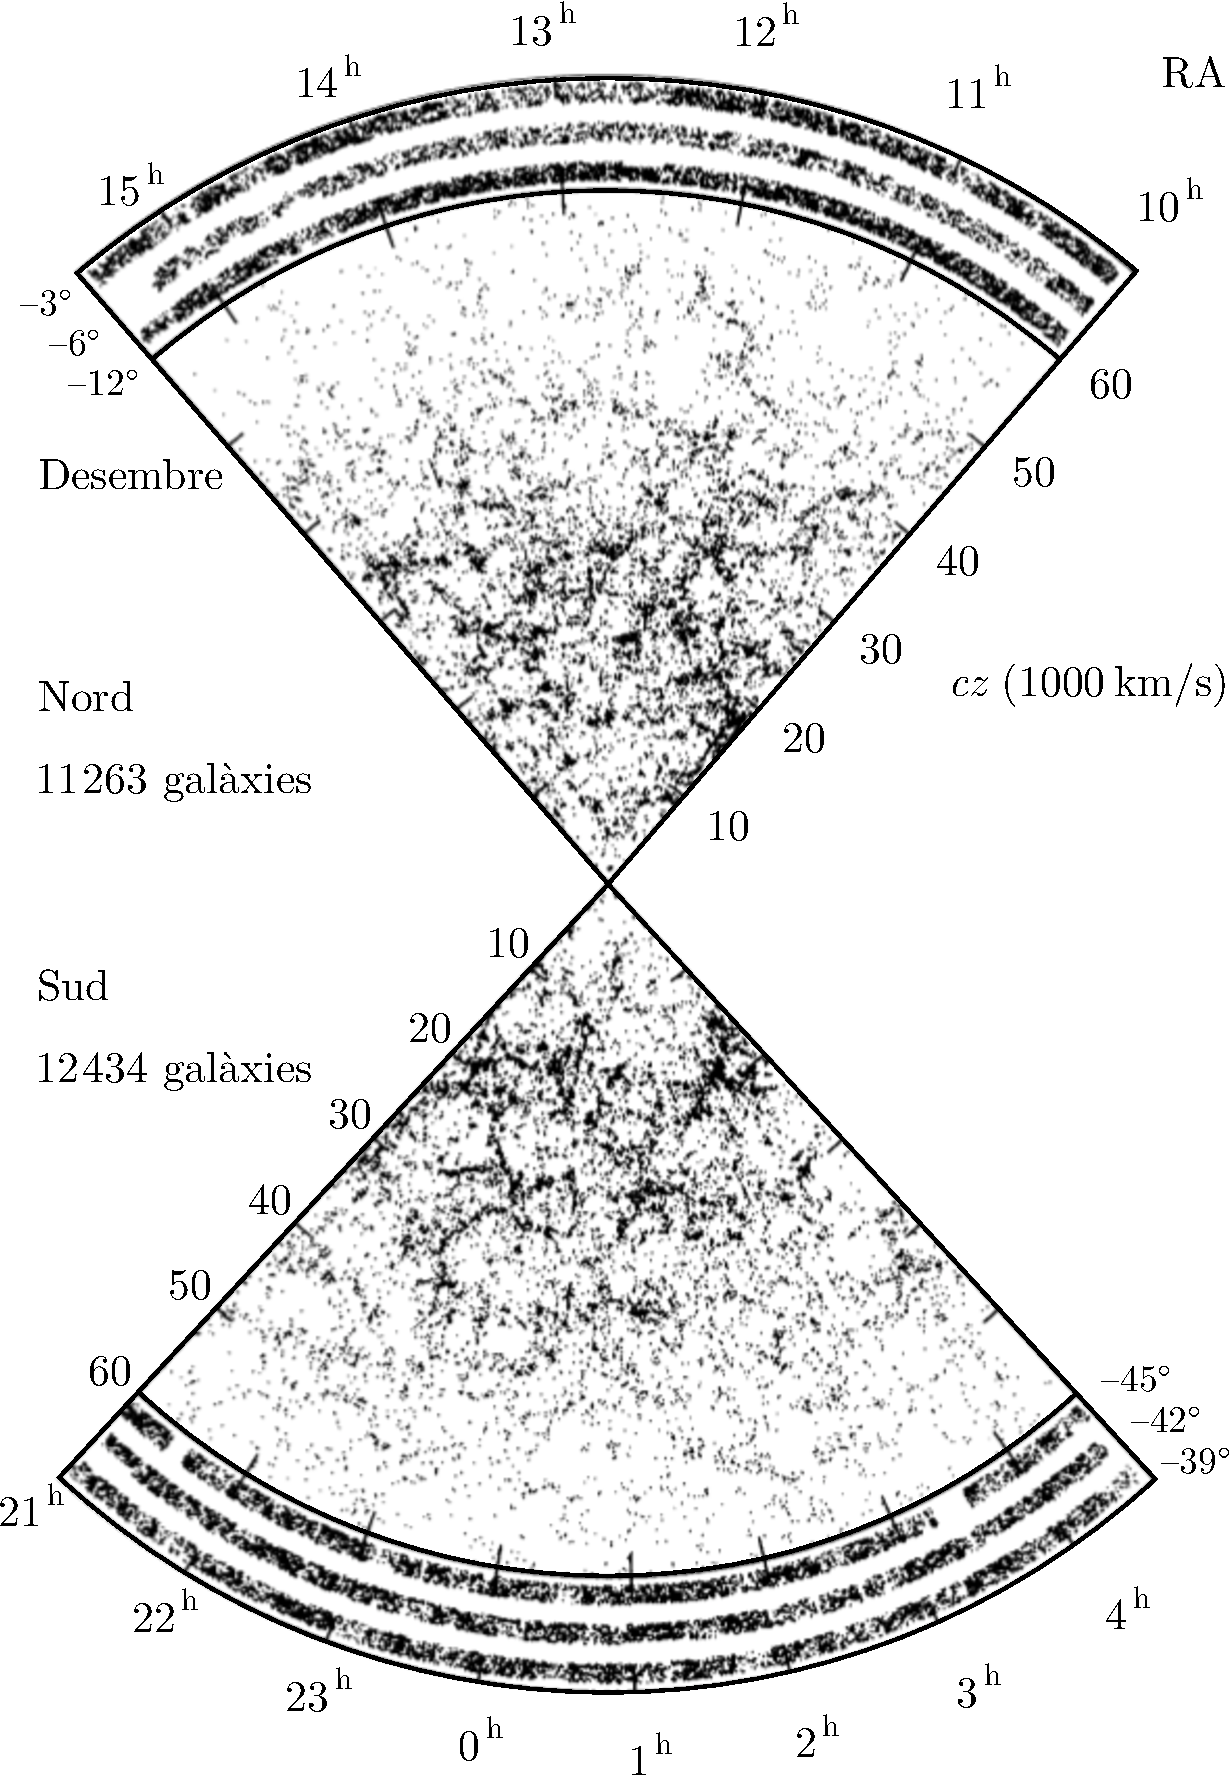
\includegraphics[width=0.7\textwidth]{./images/9-mapa-redshift}
	\caption{\textit{Redshift Survey} realitzat al \textit{Las Campanas Observatory} (LCO)} % pag 30'
	\label{fig:mapa-redshift}
\end{figure}

